% !TeX spellcheck = en_GB
% !TeX root = memoco-report.tex

\section{Tests and results}
\label{sec:results}
The described heuristic has been tested on instances generated as described in \cref{sec:datasetgen}, and its solution has been compared with the optimal solution obtained with the exact method. This has been done for instances of size up to 110, since the exact method employed too much time to solve bigger problems. In addition the same tests have been performed on some symmetric drilling problems from TSPLIB, namely \texttt{d198}, \texttt{d493} and \texttt{d657}, with respect to the optimal solutions listed at \cite{Tsplibsol}.
The parameters were set with the following values:
\begin{itemize}
	\setlength\itemsep{0.03em}
	\item K = 400 (so unbounded for size 10-110)
	\item I = 1000
	\item \texttt{max\_neighbours = 5}
	\item \texttt{backtracking\_threshold = 3}
	\item \texttt{intens\_min\_depth = 5}
	\item \texttt{intens\_n\_tours = 50}
\end{itemize}
Parameter \texttt{backtracking\_threshold} and \texttt{intens\_n\_tours} were set to a compromise between the best values found during calibration, and \texttt{intens\_min\_depth} was set to 5, since this value seemed to work best with size 90. Finally \texttt{max\_neighbours} was set to 5 because it resulted in a lower average error in both calibrations.

\subsection{Tests on syntetic dataset}
For each problem size to test, one instance was generated, and the heuristic was run on it first with 5 random restarts, then with 15 and 30. It was run 10 times for each different parameter, and the mean, standard deviation, minimum and maximum value was computed for both execution times and relative percentage error with respect to the optimal value. Tables \ref{tab:t10} - \ref{tab:t110} contains the results for some problems. Figure \ref{fig:ploterr} and \ref{fig:plotime} summarise the results for tests with 15 restarts. In addition figure \ref{fig:logtime} compares the execution times of the two methods. Here the heuristic time is the arithmetic mean of the 10 executions with 15 restarts.

% !TeX spellcheck = en_GB
% !TeX root = memoco-report.tex

\renewcommand{\arraystretch}{1.2}
%\setlength{\arrayrulewidth}{1pt}
\begin{table}[H]
	\caption{Test results on size 10}
	\label{tab:t10}
	\centering
	\begin{tabular}[t]{c|cccc|cccc}
		\rowcolor[HTML]{EFEFEF}
		& \multicolumn{4}{c|}{\textbf{Percentage relative error}} & \multicolumn{4}{c}{\textbf{Execution time}} \\
		\rowcolor[HTML]{EFEFEF}
		\textbf{Restarts} & \textbf{Mean} &\textbf{Std. dev} & \textbf{Min} & \textbf{Max} & \textbf{Mean} &\textbf{Std. dev} & \textbf{Min} & \textbf{Max} \\
		5        & 0    & 0        & 0   & 0 & \num{0.125e-2} & \num{0.127e-2} & \num{0.433e-3} & \num{0.438e-2} \\
		15       & 0    & 0        & 0   & 0 & \num{0.409e-2} & \num{0.311e-2} & \num{0.140e-2} &\num{0.974e-2} \\
		30       & 0    & 0        & 0   & 0 & \num{0.114e-1} & \num{0.445e-2} & \num{0.614e-2} & \num{0.219e-1} 
	\end{tabular}
\end{table}

\begin{table}[H]
	\caption{Test results on size 30}
	\label{tab:t30}
	\centering
	\begin{tabular}[t]{c|cccc|cccc}
		\rowcolor[HTML]{EFEFEF}
		& \multicolumn{4}{c|}{\textbf{Percentage relative error}} & \multicolumn{4}{c}{\textbf{Execution time}} \\
		\rowcolor[HTML]{EFEFEF}
		\textbf{Restarts} & \textbf{Mean} &\textbf{Std. dev} & \textbf{Min} & \textbf{Max} & \textbf{Mean} &\textbf{Std. dev} & \textbf{Min} & \textbf{Max} \\
		5        & 0    & 0        & 0   & 0 & 0.127 & \num{0.121e-1} & 0.109 & 0.149 \\
		15       & 0    & 0        & 0   & 0 & 0.407 & \num{0.616e-1} & 0.326 & 0.503 \\
		30       & 0    & 0        & 0   & 0 & 0.766 & \num{0.829e-1} & 0.669 & 0.971
	\end{tabular}
\end{table}

\begin{table}[H]
	\caption{Test results on size 50}
	\label{tab:t50}
	\centering
	\begin{tabular}[t]{c|cccc|cccc}
		\rowcolor[HTML]{EFEFEF}
		& \multicolumn{4}{c|}{\textbf{Percentage relative error}} & \multicolumn{4}{c}{\textbf{Execution time}} \\
		\rowcolor[HTML]{EFEFEF}
		\textbf{Restarts} & \textbf{Mean} &\textbf{Std. dev} & \textbf{Min} & \textbf{Max} & \textbf{Mean} &\textbf{Std. dev} & \textbf{Min} & \textbf{Max} \\
		5        & 0    & 0        & 0   & 0 & 0.139 & \num{0.205e-1} & 0.119 & 0.179 \\
		15       & 0    & 0        & 0   & 0 & 0.448 & \num{0.791e-1} & 0.347 & 0.605 \\
		30       & 0    & 0        & 0   & 0 & 0.897 & \num{0.914e-1} & 0.784 & \num{0.105e+1}
	\end{tabular}
\end{table}

\begin{table}[H]
	\caption{Test results on size 70}
	\label{tab:t70}
	\centering
	\begin{tabular}[t]{c|cccc|cccc}
		\rowcolor[HTML]{EFEFEF}
		& \multicolumn{4}{c|}{\textbf{Percentage relative error}} & \multicolumn{4}{c}{\textbf{Execution time}} \\
		\rowcolor[HTML]{EFEFEF}
		\textbf{Restarts} & \textbf{Mean} &\textbf{Std. dev} & \textbf{Min} & \textbf{Max} & \textbf{Mean} &\textbf{Std. dev} & \textbf{Min} & \textbf{Max} \\
		5        & 0    & 0        & 0   & 0 & 0.418 & \num{0.469e-1} & 0.331 & 0.479 \\
		15       & 0    & 0        & 0   & 0 & \num{0.121e+1} & \num{0.607e-1} & \num{0.109e+1} & \num{0.130e+1} \\
		30       & 0    & 0        & 0   & 0 & \num{0.241e+1} & 0.109 & \num{0.226e+1} & \num{0.264e+1}
	\end{tabular}
\end{table}

\begin{table}[H]
	\caption{Test results on size 80}
	\label{tab:t80}
	\centering
	\begin{tabular}[t]{c|cccc|cccc}
		\rowcolor[HTML]{EFEFEF}
		& \multicolumn{4}{c|}{\textbf{Percentage relative error}} & \multicolumn{4}{c}{\textbf{Execution time}} \\
		\rowcolor[HTML]{EFEFEF}
		\textbf{Restarts} & \textbf{Mean} &\textbf{Std. dev} & \textbf{Min} & \textbf{Max} & \textbf{Mean} &\textbf{Std. dev} & \textbf{Min} & \textbf{Max} \\
		5        & 0.192& 0.236& 0   & 0.481  & 0.617 & 0.167 & 0.427 & \num{0.108e+1} \\
		15       & 0    & 0        & 0   & 0  & \num{0.183e+1} & 0.178 & \num{0.148e+1} & \num{0.213e+1} \\
		30       & 0    & 0        & 0   & 0  & \num{0.374e+1} & 0.291 & \num{0.332e+1} & \num{0.420e+1}
	\end{tabular}
\end{table}


\begin{table}[H]
	\caption{Test results on size 100}
	\label{tab:t100}
	\centering
	\begin{tabular}[t]{c|cccc|cccc}
		\rowcolor[HTML]{EFEFEF}
		& \multicolumn{4}{c|}{\textbf{Percentage relative error}} & \multicolumn{4}{c}{\textbf{Execution time}} \\
		\rowcolor[HTML]{EFEFEF}
		\textbf{Restarts} & \textbf{Mean} &\textbf{Std. dev} & \textbf{Min} & \textbf{Max} & \textbf{Mean} &\textbf{Std. dev} & \textbf{Min} & \textbf{Max} \\
		5        & 0.320    & 0.209  & 0.128   & 0.769 & 0.950 & 0.160 & 0.689 & \num{0.125e+1} \\
		15       & 0.128    & 0.152  & 0   & 0.513  & \num{0.277e+1} & 0.237 & \num{0.246e+1} & \num{0.337e+1} \\
		30       & \num{0.769e-1}    & \num{0.628e-1} & 0   & 0.128 & \num{0.577e+1} & 0.526 & \num{0.518e+1} & \num{0.722e+1}  
	\end{tabular}
\end{table}

\begin{table}[H]
	\caption{Test results on size 110}
	\label{tab:t110}
	%\setlength\tabcolsep{5pt}
	\centering
	\begin{tabular}[t]{c|cccc|cccc}
		\rowcolor[HTML]{EFEFEF}
		& \multicolumn{4}{c|}{\textbf{Percentage relative error}} & \multicolumn{4}{c}{\textbf{Execution time}} \\
		\rowcolor[HTML]{EFEFEF}
		\textbf{Restarts} & \textbf{Mean} &\textbf{Std. dev} & \textbf{Min} & \textbf{Max} & \textbf{Mean} &\textbf{Std. dev} & \textbf{Min} & \textbf{Max} \\
		5        & 0.484    & 0.254  & 0   & 0.806 & \num{0.129e1} & 0.145 & \num{0.106e+1} & \num{0.155e+1} \\
		15       & 0.202    & 0.197  & 0   & 0.504  & \num{0.418e+1} & 0.390 & \num{0.360e+1} & \num{0.514e+1} \\
		30       & \num{0.806e-1}    & 0.134 & 0   & 0.403 & \num{0.831e+1} & 0.604 & \num{0.740e+1} & \num{0.929e+1}
	\end{tabular}
\end{table}

\begin{figure}[H]
	\centering
	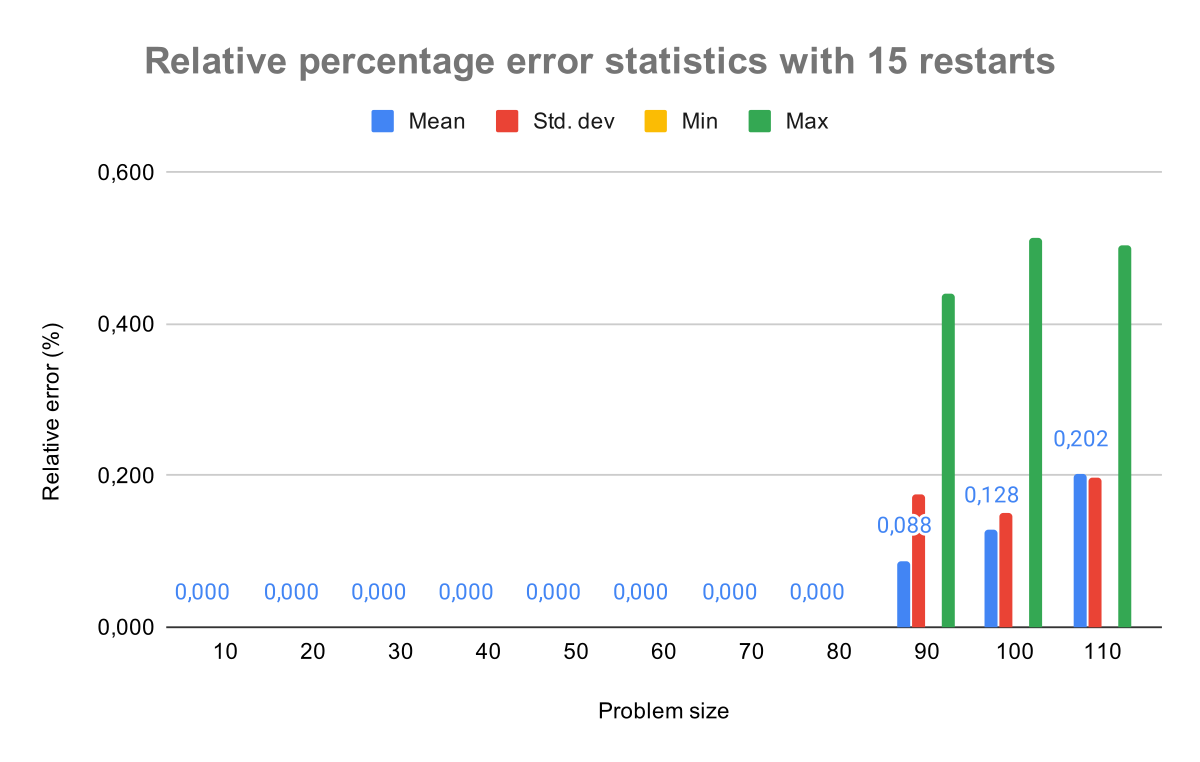
\includegraphics[width=0.9\textwidth]{error_plot}
	\caption{Error statistics over 10 runs with 15 restarts}
	\label{fig:ploterr}
\end{figure}

\begin{figure}[H]
	\centering
	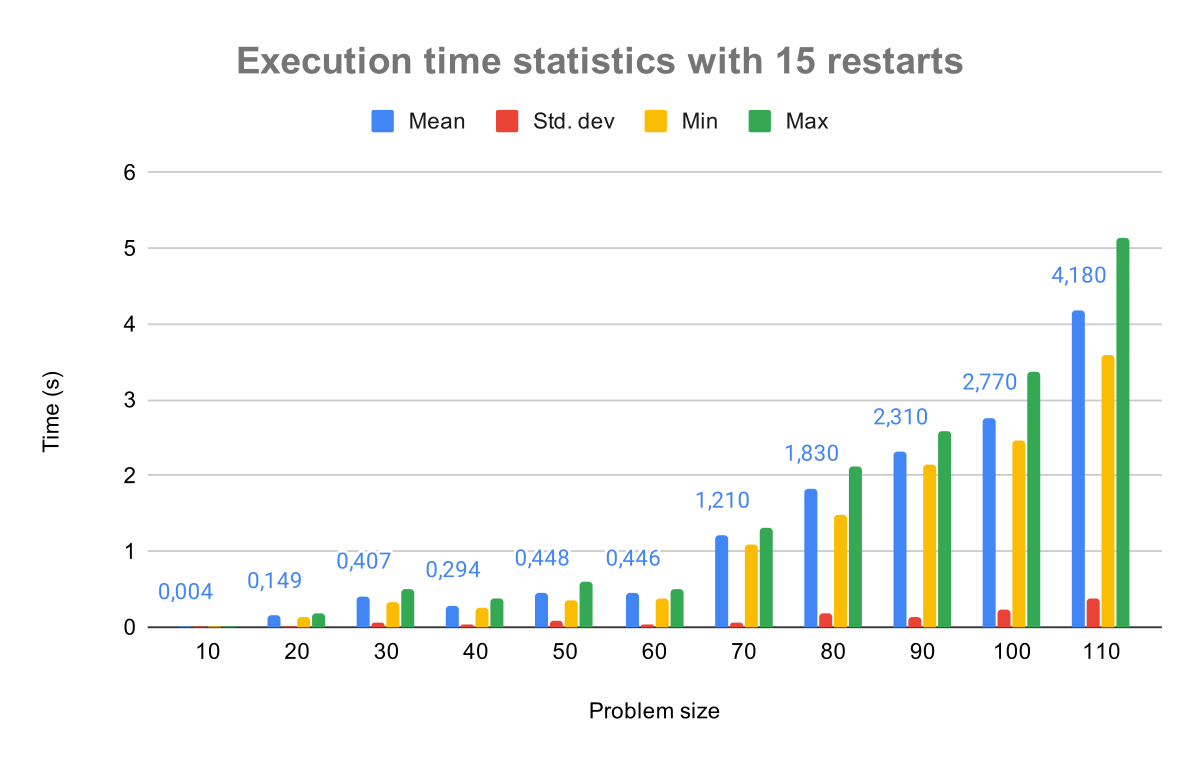
\includegraphics[width=0.9\textwidth]{time_plot}
	\caption{Execution time statistics over 10 runs with 15 restarts}
	\label{fig:plotime}
\end{figure}

\begin{figure}[H]
	\centering
	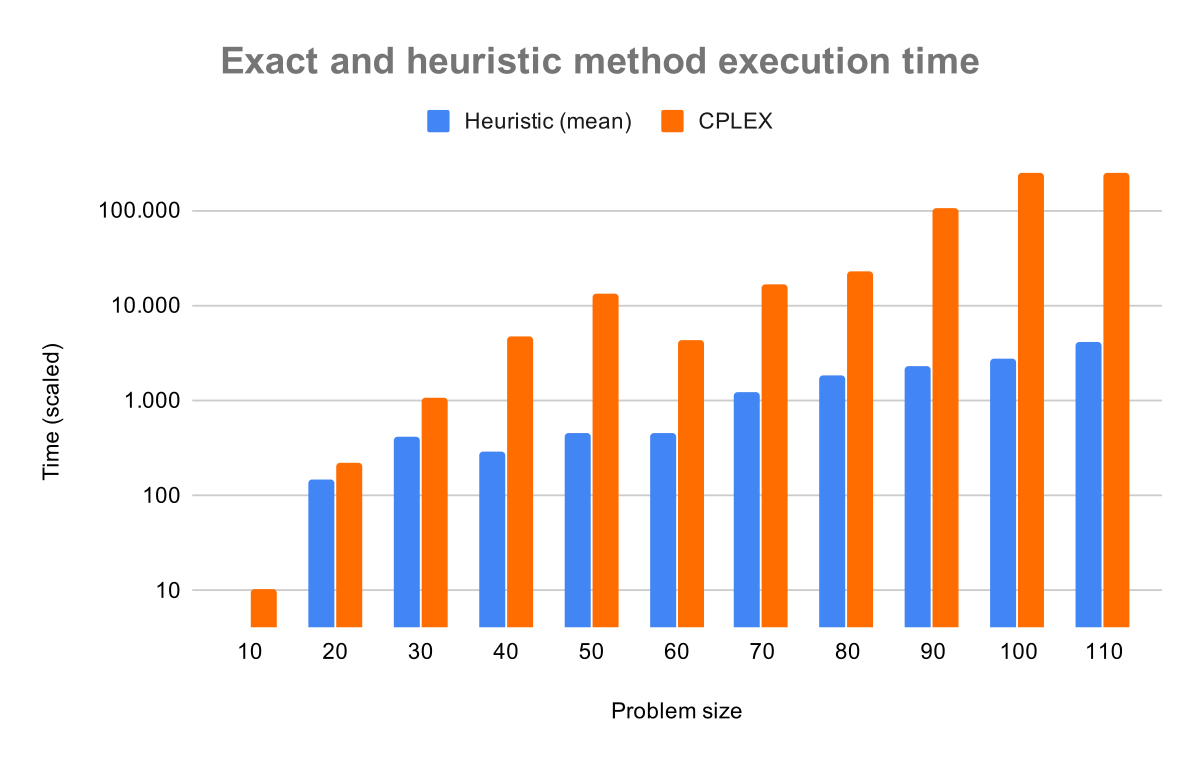
\includegraphics[width=.9\textwidth]{logtime_plot}
	\caption{Comparison of execution times for both methods (multiplied by 1000, logarithmic scale)}
	\label{fig:logtime}
\end{figure}

\subsection{Tests on bigger instances}
Table \ref{tab:tsplibr} lists the results of testing the heuristic method with some bigger instances taken from TSPLIB. Extensive tests would require much time, so these results come from a single execution of the heuristic with the same parameters used for previous tests, but with 30 restarts instead of 15. For problem \texttt{d657} parameter \texttt{backtracking\_threshold} was lowered to 2 to reduce running time.  The produced solution paths are shown in figures \ref{fig:p198}, \ref{fig:p493} and \ref{fig:p657}.

\begin{table}[h]
	\caption{Results on TSPLIB problems}
	\label{tab:tsplibr}
	\centering
	\begin{tabular}[t]{cccccc}
		\rowcolor[HTML]{EFEFEF}
		\textbf{Problem} & \textbf{Size} & \textbf{Optimal value} & \textbf{Heuristic value} & \textbf{Relative error (\%)} & \textbf{Time (s)} \\
		d198    & 198 & 15780 & 15852.9 & 0.462  & 266   \\
		d493    & 493 & 35002 & 35428.1 & 1.217 & 3638	\\
		d657 *	& 657 & 48912 & 49892.1 & 2.004	&  2032 \\
		\multicolumn{6}{l}{\rule{0pt}{4ex}*\texttt{backtracking\_threshold = 2}} 
	\end{tabular}
\end{table}

\begin{figure}[H]
	\centering
	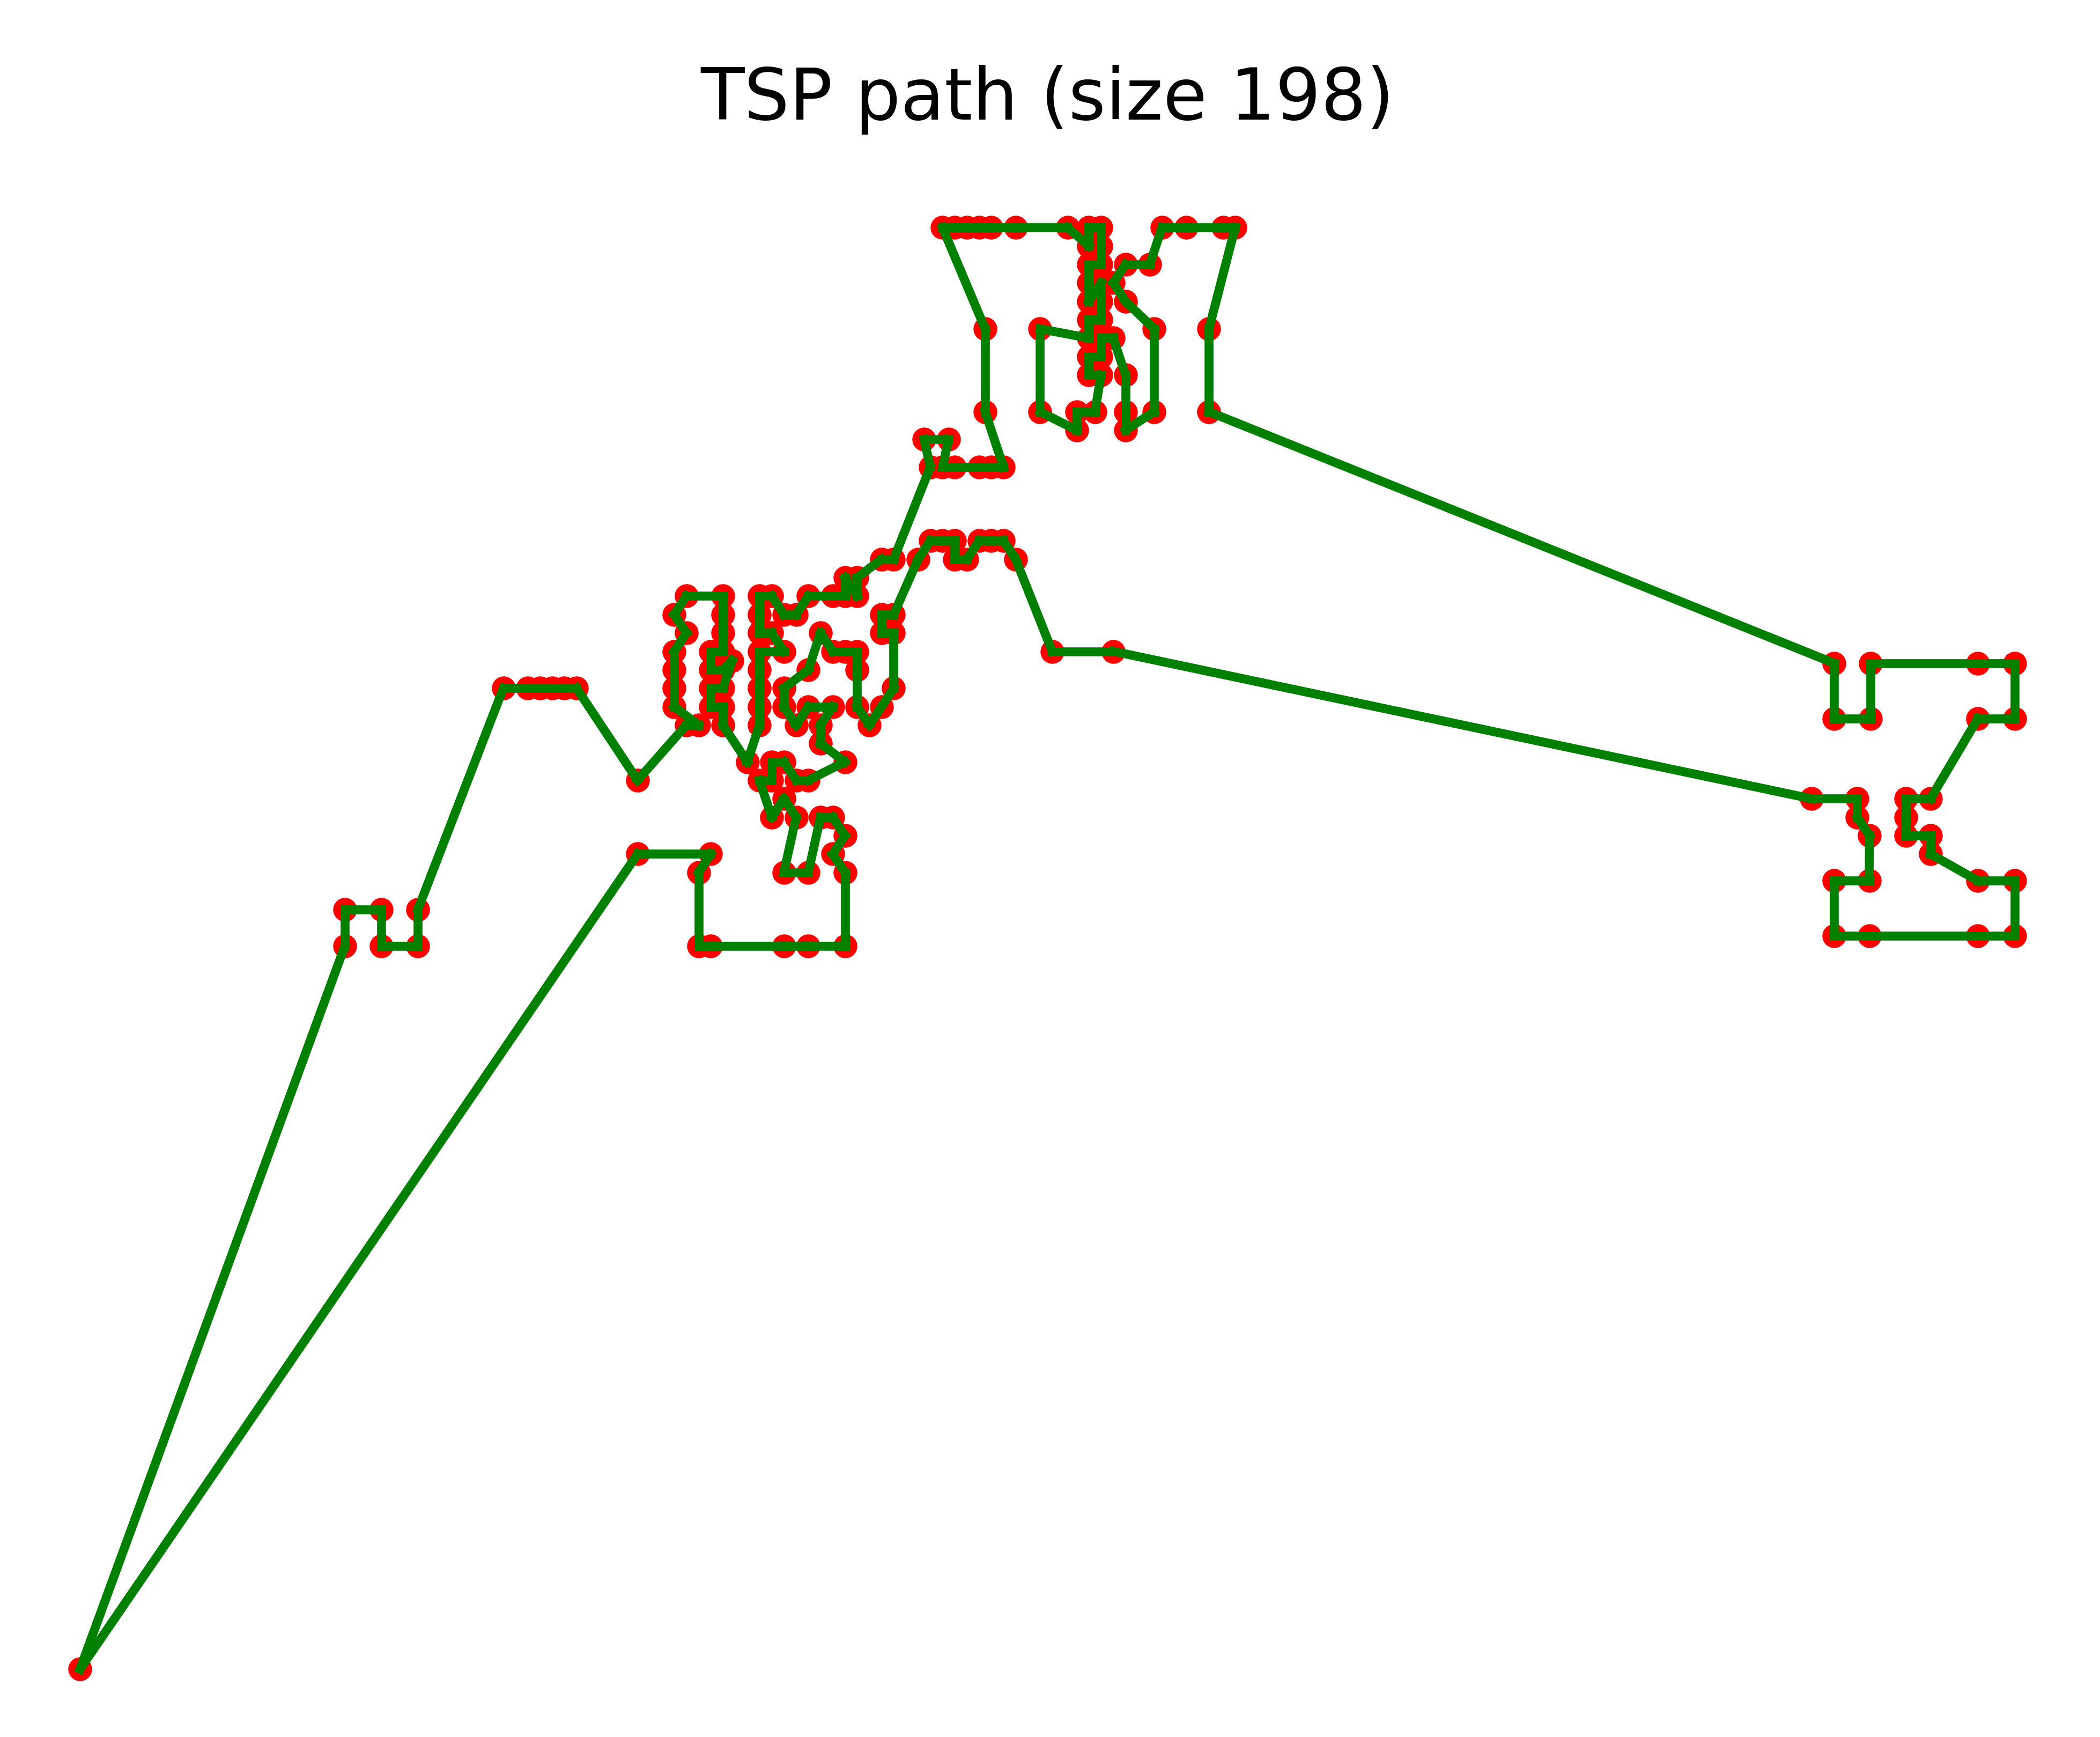
\includegraphics[width=12cm]{path_198}
	\caption{Heuristic solution for d198}
	\label{fig:p198}
\end{figure}

\begin{figure}[H]
	\centering
	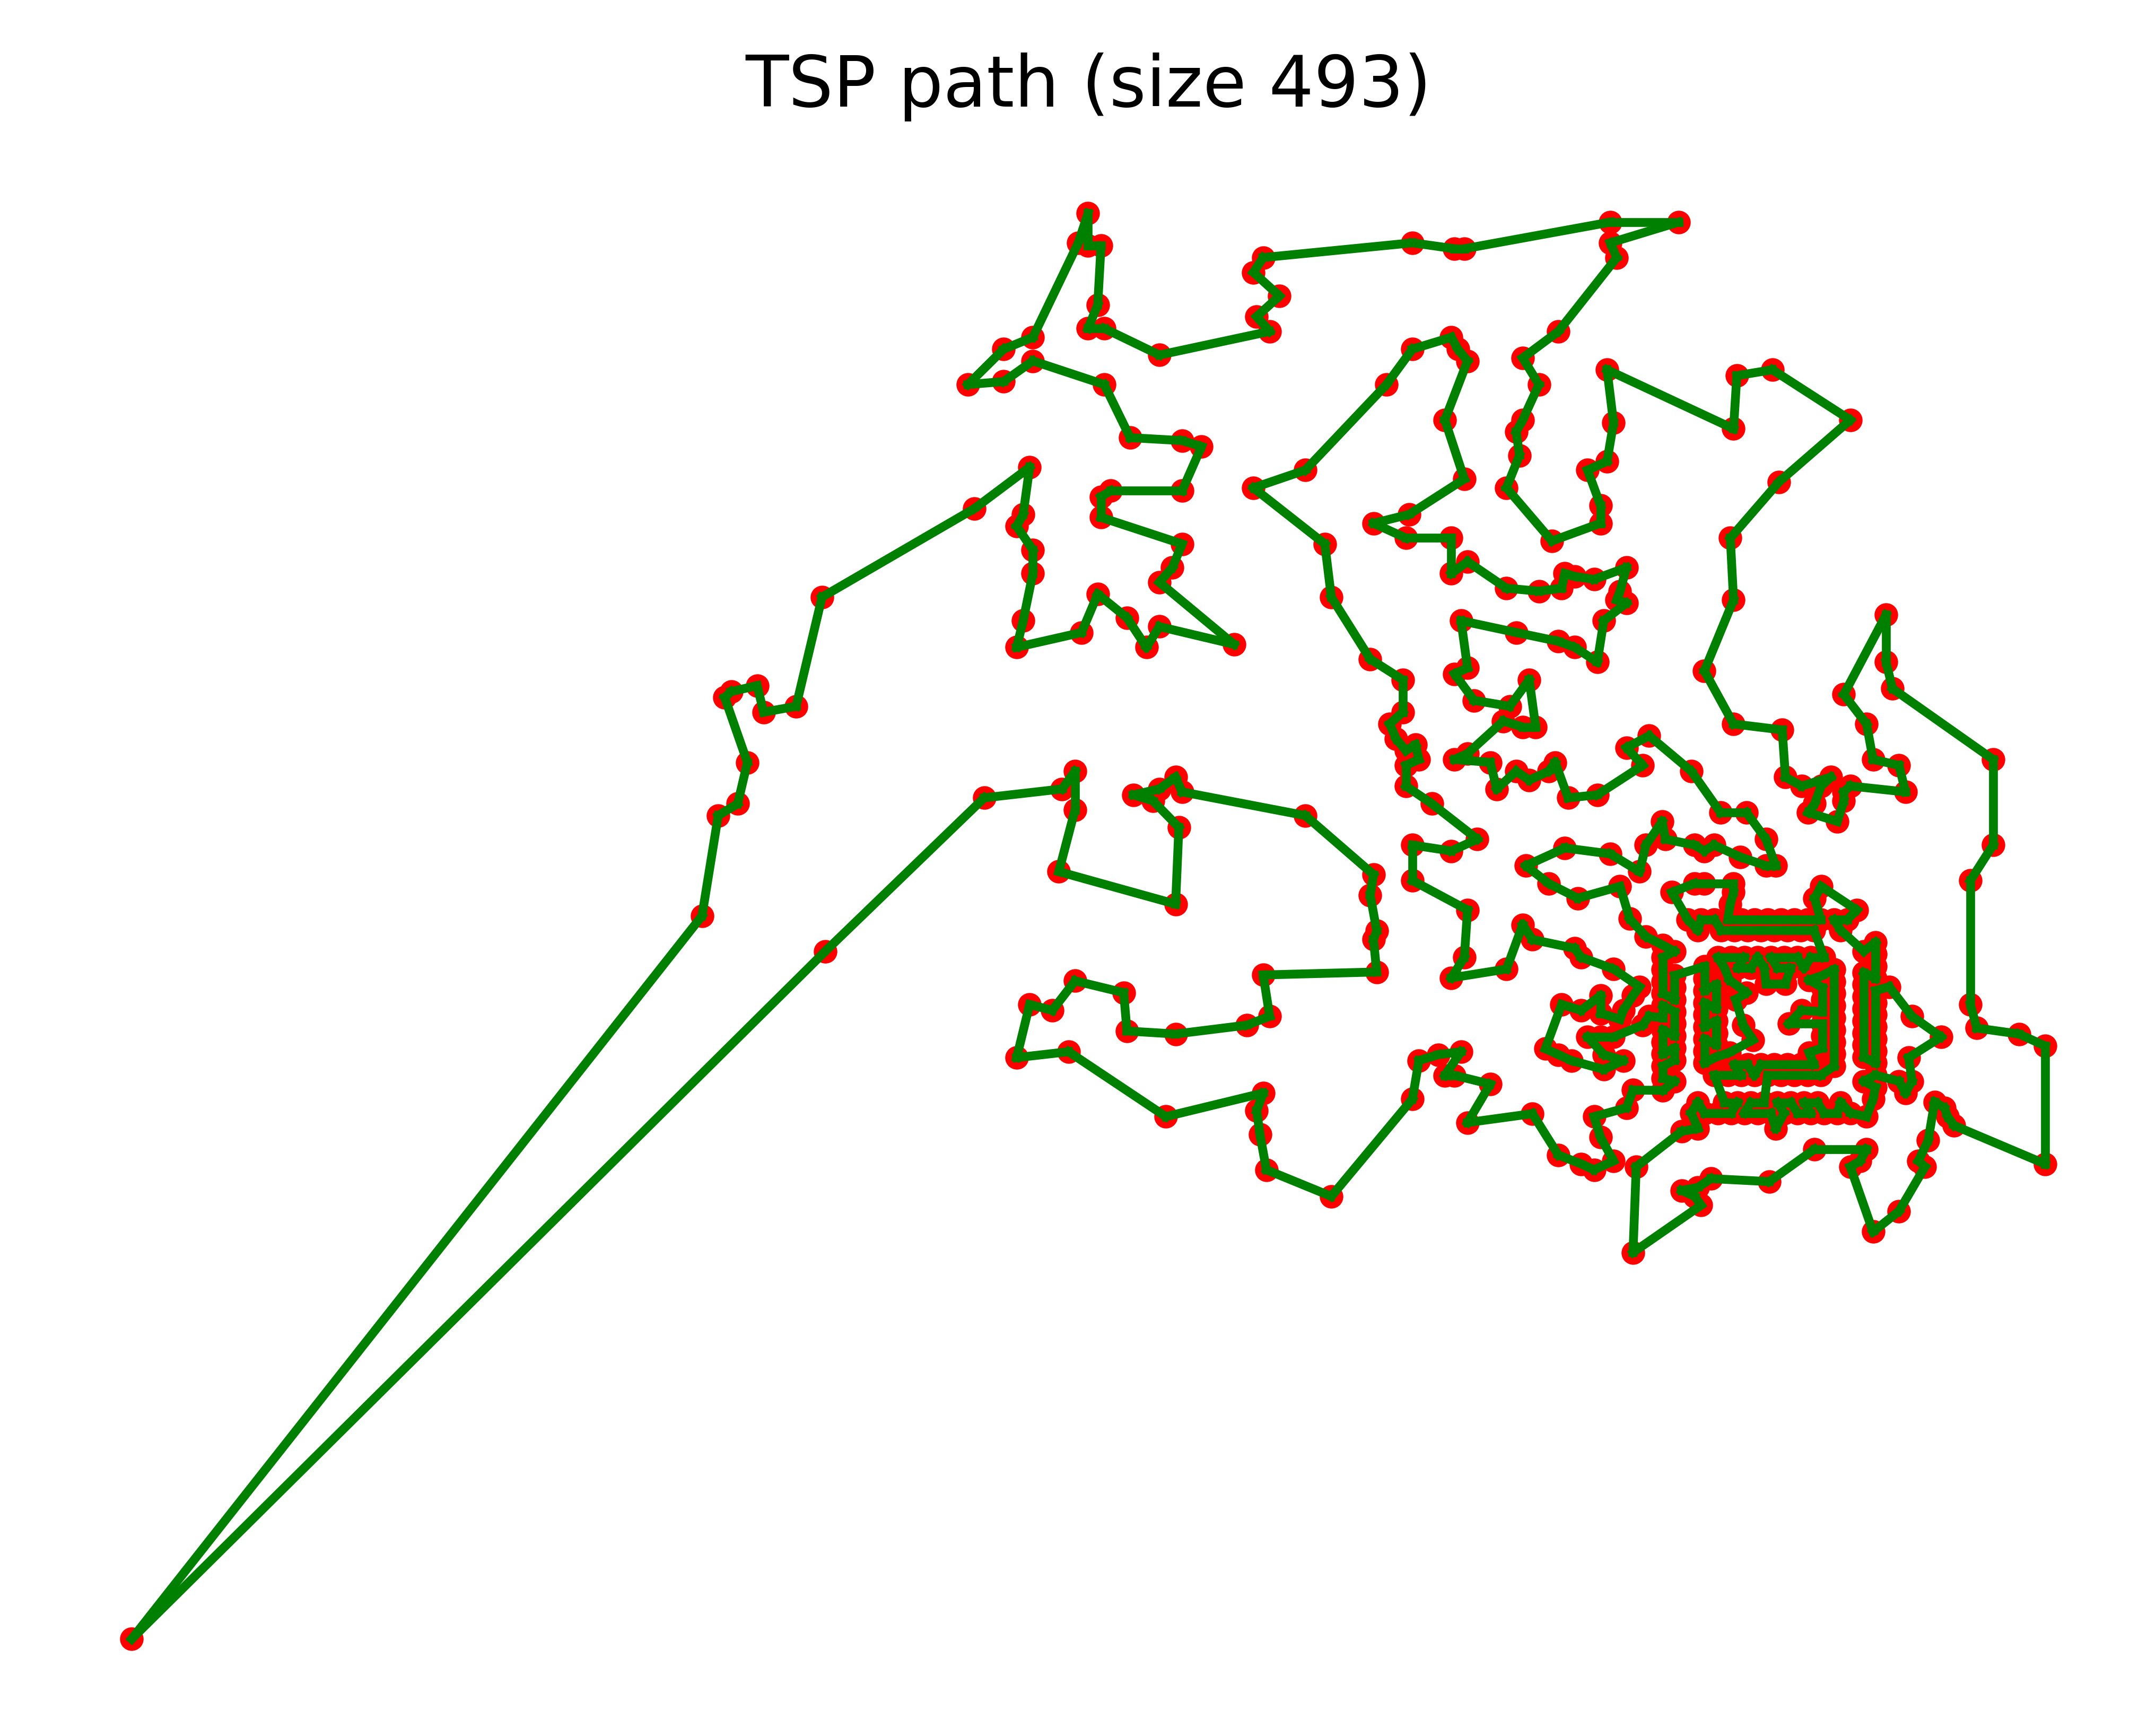
\includegraphics[width=12cm]{path_493}
	\caption{Heuristic solution for d493}
	\label{fig:p493}
\end{figure}

\begin{figure}[H]
	\centering
	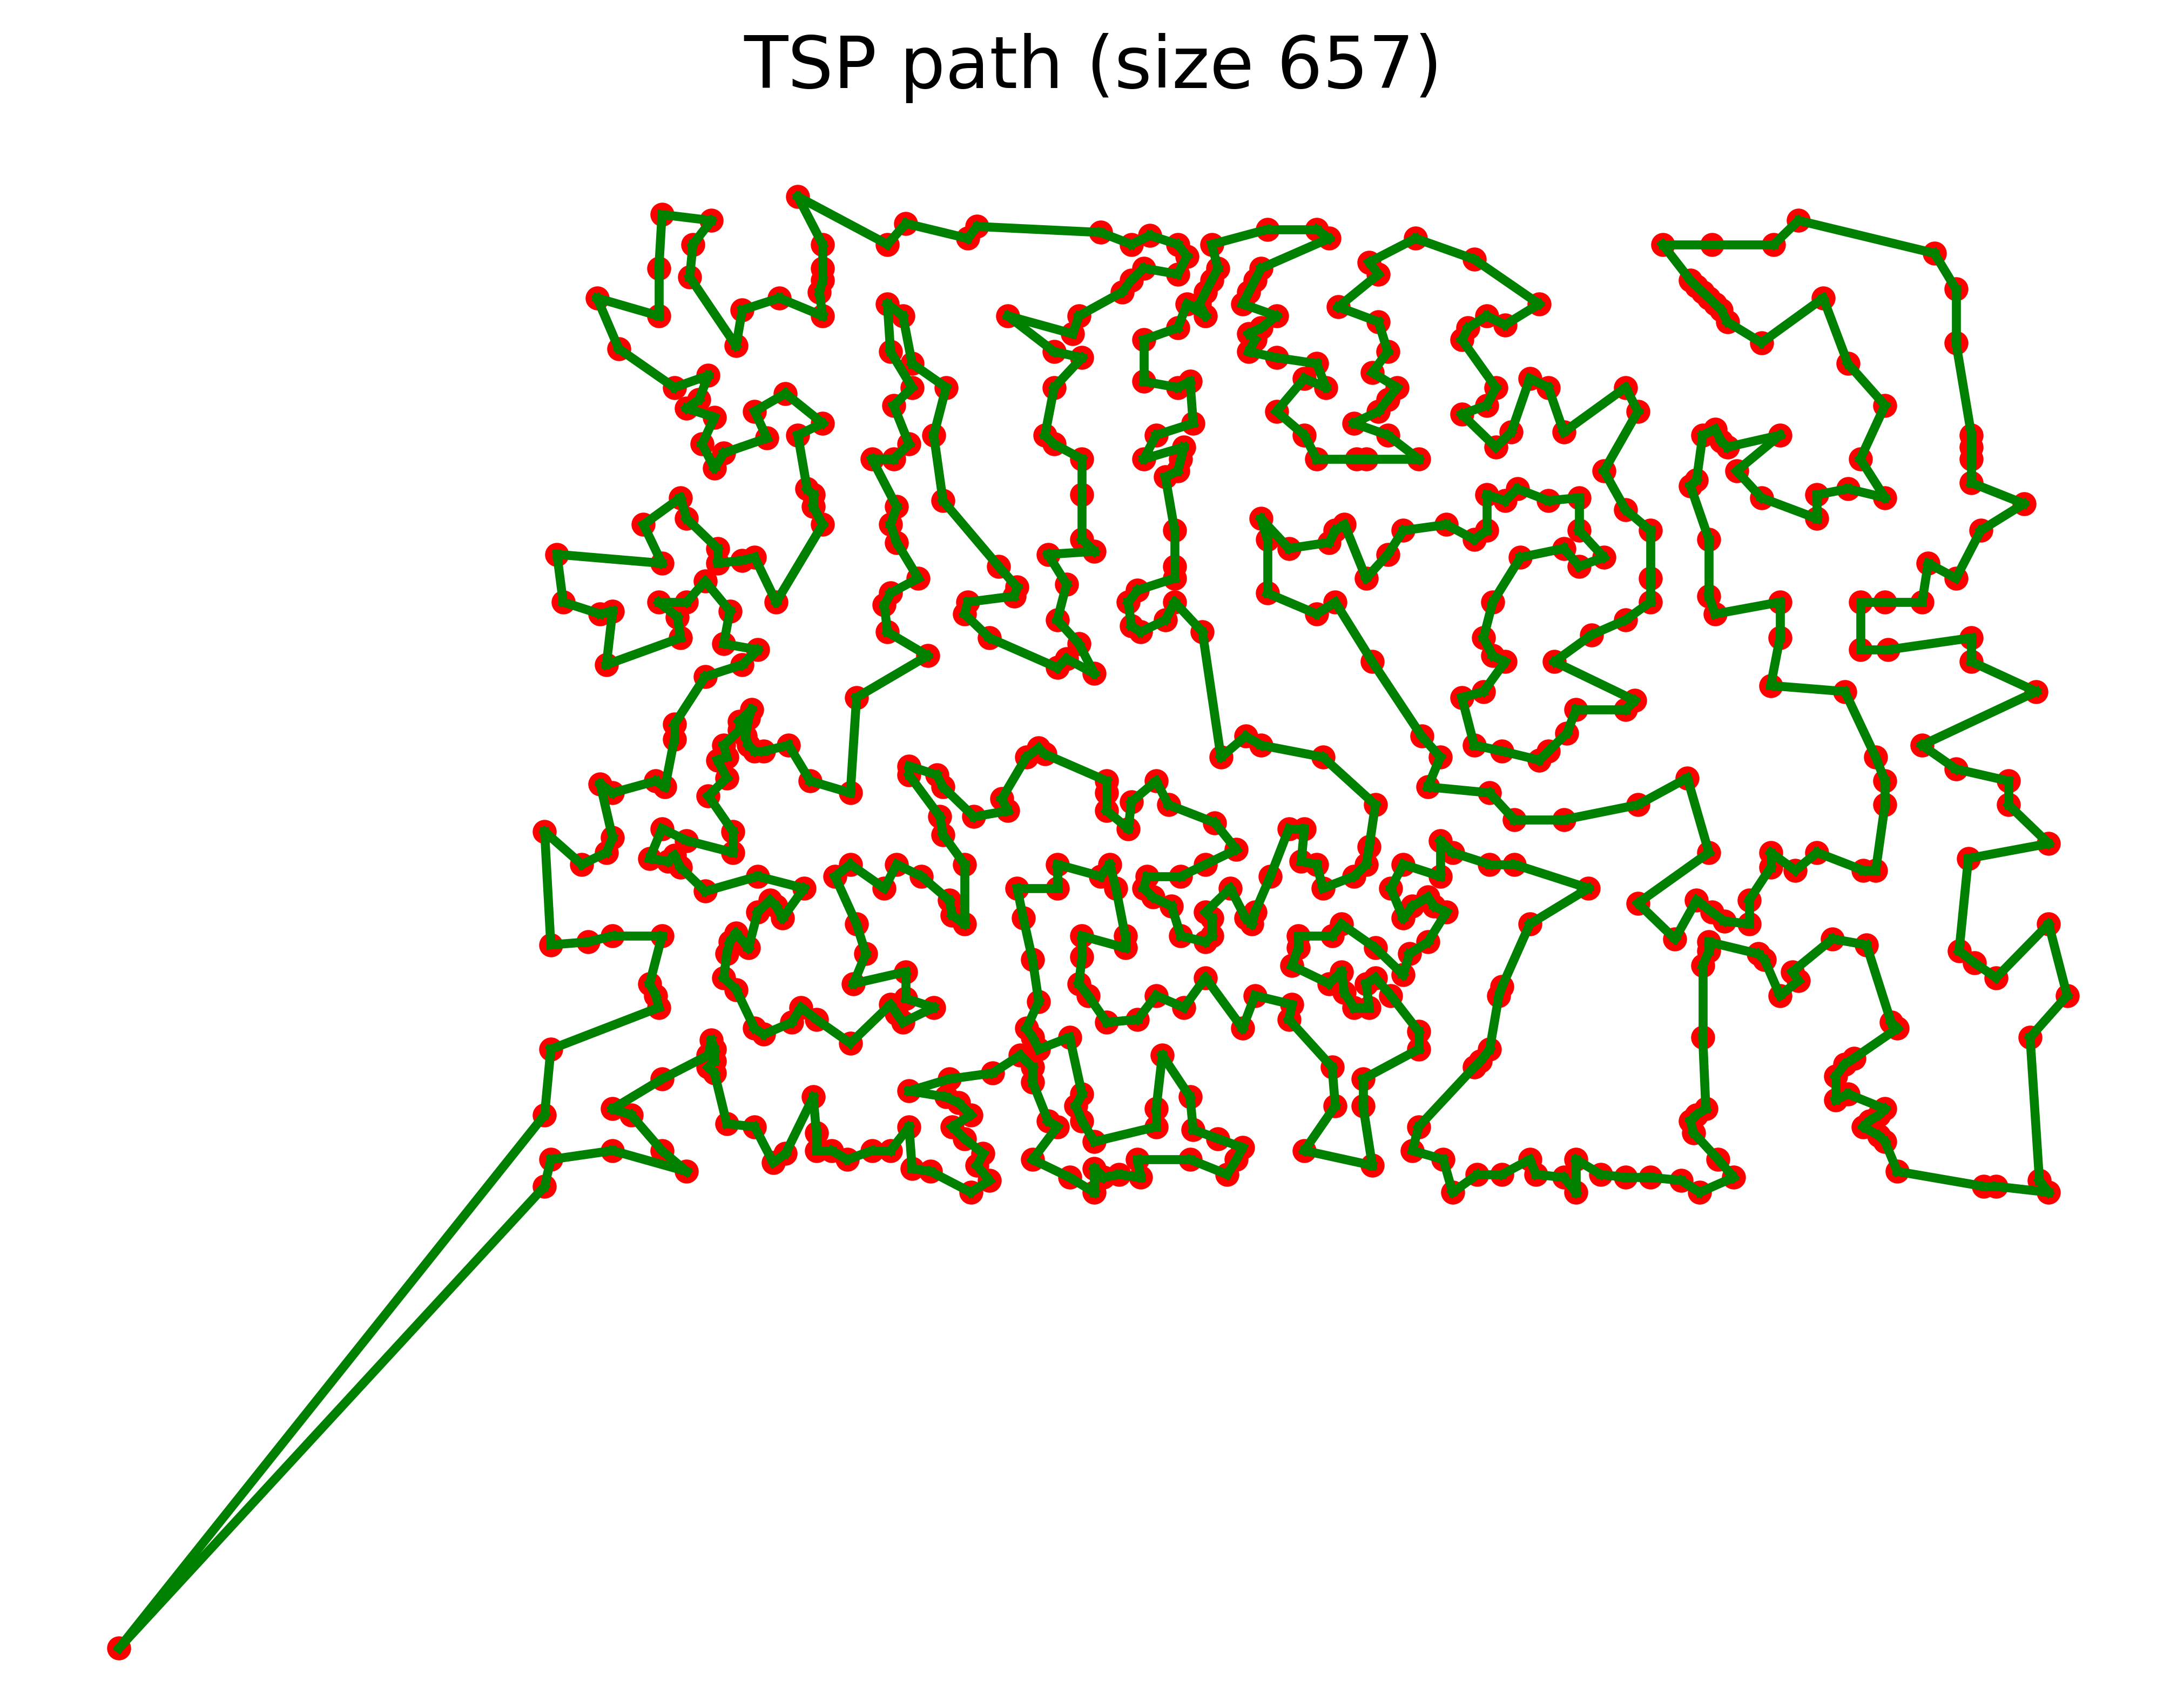
\includegraphics[width=12cm]{path_657}
	\caption{Heuristic solution for d657}
	\label{fig:p657}
\end{figure}


